\documentclass[12pt]{tcc}
\usepackage[brazil]{babel}
\usepackage[T1]{fontenc}
%\usepackage[brazilian,hyperpageref]{backref}
\usepackage[hidelinks]{hyperref}
\usepackage[pt-BR]{datetime2}
\DTMlangsetup{showdayofmonth=false}
\usepackage[portuguese,ruled,linesnumbered,algochapter,titlenumbered]{algorithm2e}
\usepackage{listings}
\usepackage{xcolor}
\usepackage[toc,page]{appendix}
\definecolor{mygreen}{RGB}{64,100,64}

% Define TypeScript language style
\lstdefinelanguage{TypeScript}{
    keywords=[1]{import, from, export, static, public, implements, extends, class, extends, private, void, constructor, super, this, async, await, for, of, let, in, return, console, log, abstract},
    keywordstyle=[1]\color{blue},
    keywords=[3]{MockTime, Promise, IPersister, Task, CompositeTask, BasicPersister, Resource, Project, MockTask, Metric, DeltaTimeMetric, ProcessMemoryMetric, Set, JSON, Math, any, string},
    keywordstyle=[3]\color{mygreen},
    ndkeywords={true, false, catch, function, null, undefined},
    ndkeywordstyle=\color{darkgray},
    identifierstyle=\color{black},
    sensitive=true,
    comment=[l]{//},
    morecomment=[s]{/*}{*/},
    commentstyle=\color{green}\ttfamily,
    stringstyle=\color{red}\ttfamily,
    morestring=[b]',
    morestring=[b]",
	lineskip=-1pt
}

\lstset{
    backgroundcolor=\color[gray]{0.9},
    numbers=left,
    stepnumber=1,
    numberstyle=\small\ttfamily\color{gray},
    numbersep=5pt,
    aboveskip=10pt,
    belowskip=10pt
}

% As figuras ficam armazenadas na pasta figuras
\graphicspath{{./figures/}}

% Informações do trabalho
\newcommand\dtitle{Framework para Análise de Desempenho de Consultas Web}
\newcommand\dauthor{Filipe Shanom Glathardt de Azeredo Xavier\\Matheus dos Santos Moura\\Radhanama Dasa de Maria Moraes Mesiano}
\newcommand\dadvisor{Renato Campos Mauro}

% Definição de acronimos
\newacro{TCC}{Trabalho de Conclusão de Curso}
\newacro{QoS}{qualidade de serviço}
\newacro{API}{\emph{Application Programming Interface}}

\begin{document}
\pagenumbering{gobble}
\pagenumbering{roman}

\dcover

\dcoverback
	
\dlibrary{ficha.pdf}
		
\ddedicatory{
	\raggedleft \normalsize Dedico este trabalho aos futuros pesquisadores, cuja as descobertas e avanços sejam impulsionados por esse trabalho. Que esse framework sirva de apoio para que possam avaliar o desempenho de suas próximas pesquisas, e que isso gere impactos positivos na sociedade.
	Dedicamos também aos nossos professores, cuja orientação nos trouxe os conhecimentos necessários para realização desse projeto. Seus ensinamentos foram fundamentais para nos capacitar a desenvolver esse trabalho.
}

\dacknowledgment{
	Agradece-se à CAPES, CNPq e FAPERJ pelo financiamento parcial desta pesquisa.\\
	\\
	Agradece-se também à plataforma Scopus e à CAPES pelas valiosas fontes de pesquisa que foram extremamente importantes para a fundação teórica deste trabalho. 
	Também desejo expressar minha gratidão aos meus colegas de grupo, cuja colaboração e esforço conjunto foram fundamentais em todas as etapas do projeto. A colaboração de cada um de vocês foi de extrema importância.
	Por fim, não podemos deixar de agradecer aos nossos familiares, cujo apoio, encorajamento e compreensão nos motivaram a superar os desafios propostos.
}

\dresumo{
Desde a popularização dos smartphones a quantidade de dados gerados cresce sem precedentes, de modo que até torna a definição de grande volume de dados difícil, devido a sua rápida obsolescência.
Dentro deste contexto, aplicações Web cliente-servidor as quais ofertam visualização de dados para grandes volumes sofrem muitas vezes com limitações de recursos computacionais no lado do cliente.
Além disso, seus desenvolvedores encontram desafios ao avaliar o consumo dos recursos, pois, há grandes dificuldades em cobrir a ampla gama de configurações que existem no lado do cliente.
Por outro lado, também existe uma carência por ferramentas as quais permitam esse tipo de avaliação, e que possuam funcionalidades para auxiliar a coleta de métricas de execuções da aplicação realizadas por voluntários.
A fim de solucionar estes problemas, propomos um framework para o ecossistema JavaScript capaz de executar provas de conceito, enquanto realiza a coleta de métricas de desempenho e consumo de recursos computacionais, o qual também seja facilmente extensível para necessidades específicas do projeto e que auxilie no processo de avaliação realizado por voluntários.
}{big data; Web; visualização de dados; avaliação de desempenho; consumo de recursos; framework}

\dabstract{
Since the popularization of smartphones, the amount of data generated has grown unprecedentedly, so that it even makes it difficult to define how big big data is, due to its rapid obsolescence.
In this context, client-server Web applications which offer data visualization for big data often suffer from limitations of computational resources on the client side.
In addition, its developers find challenges when evaluating resource consumption, as there are great difficulties in covering a wide range of configurations on the client side.
On the other hand, there is also a lack of tools that guarantee this type of evaluation, and contain features to help collect application execution metrics performed by volunteers.
In order to solve these problems, we propose a framework for the JavaScript ecosystem capable of executing proofs of concept, while collecting performance indicators and consumption of computational resources, which is also easily extensible for specific needs of the project and that helps the estimation process carried out by volunteers.
}{big data; Web; data visualization; performance evaluation; resource consumption; framework}

\dtables
	

\pagenumbering{arabic}
\justifying
	
\chapter{Introdução}
\label{cap:intro}

Desde o começo da era da informação e principalmente após a popularização dos smartphones a quantidade de informações geradas cresce em um ritmo sem precedentes \citep{Gandomi2015Beyond}.
Este cenário com disponibilidade de grandes volumes de dados (do inglês, \emph{big data}), criou diversas oportunidades para modelos de negócios voltados para o uso desses dados.
Empresas como Google e Meta (antigo Facebook), se tornaram gigantes do mercado explorando estes modelos de negócios baseados em dados.

Entretanto, o manuseio de grandes volumes de dados necessita de cuidados especiais.
Pois, eles podem superar o tamanho de qualquer memória principal ou secundária as quais são encontradas no mercado.
Alguns exemplos desses tratamentos especiais para o manuseio de grandes volumes de dados são o modelo de programação MapReduce \citep{Dean2008MapReduce} e o sistema de armazenamento de objetos Haystack \citep{Beaver2010Finding}.
Portanto, os sistemas que manuseiam grandes volumes de dados precisam ser planejados para sua carga de trabalho.

Por outro lado, aplicações Web com arquitetura cliente-servidor sofrem com o problema da ampla variedade de configurações tanto de hardware quanto de software no lado do cliente.
E, os desenvolvedores, por sua vez, não possuem diversos tipos de ambientes para exercitar suas aplicações, o que pode levar a problemas com alguns tipos de configurações.
Além disso, mesmo quando existe acesso a diferentes tipos de ambiente, é improvável que a equipe de desenvolvimento tenha acesso direto, sendo necessário a colaboração de alguém externo.

A fim de atenuar estes problemas, estamos propondo um framework o qual um desenvolvedor de uma aplicação Web cliente-servidor seja capaz de facilmente obter métricas e estatísticas sobre provas de conceito, as quais, precisam ser executadas em diversas configurações de clientes por voluntários.
Por exemplo, considere uma aplicação Web a qual precisa trafegar um volume suficientemente grande de dados entre o cliente e o servidor, de modo que, seja impossível de manter todos dados em cache no lado do cliente.

Para realizar o tráfego de dados, a equipe de desenvolvimento considera as seguintes opções de formato de arquivo: CSV, JSON, Arrow e Parquet.
Com o objetivo de tomar essa decisão, a equipe decide realizar uma análise de desempenho e consumo de recursos em cada uma das abordagens variando os tipos de clientes.
E, para incluir nas avaliações a maior variedade possível de clientes, eles também decidem automatizá-la, de modo que seja possível contar com o auxílio de voluntários.
Porém, com o intuito de tornar isso possível, além da prova de conceito, a equipe ainda precisaria desenvolver como expor, executar e coletar as métricas durante a avaliação.

Este é o tipo de cenário para qual o framework está sendo proposto.
Por disponibilizar uma aplicação Web pronta e capaz de envolver provas de conceito, automatizar sua execução, coletar métricas e ser de fácil extensão.
Ademais, o framework por padrão possui as métricas básicas implementadas, como tempo gasto na tarefa, memória utilizada, identificação do ambiente de execução e os dados são armazenados em uma planilha online para fácil obtenção e análise.
Deste modo, o desenvolvedor pode focar nas provas de conceito e na obtenção de ambientes e voluntários, ao invés do desenvolvimento de infraestrutura para realização das avaliações.

Além disso, o trabalho está dividido em cinco capítulos.
O capítulo \ref{cap:met_pesquisa} e \ref{sec:trab_relacionados} correspondem a metodologia da pesquisa e trabalhos relacionados encontrados no campo de estudo.
O capítulo \ref{cap:proposta} apresenta a proposta de desenvolvimento da ferramenta.
Por fim, os capítulos \ref{cap:prova_de_conceito} e \ref{cap:estado_atual} apresenta o estado atual do framework e o cronograma para a próxima etapa.


\chapter{Metodologia da Pesquisa}
\label{cap:met_pesquisa}

Para a revisão bibliográfica as duas principais ferramentas utilizadas foram: Elicit, um assistente de pesquisa baseado em modelos de transformador pré-treinado generativo (do inglês, \emph{generative pre-trained transformer}) de aprendizado de máquina, e a ferramenta Connected Papers, a qual  gera um grafo de artigos relacionados baseado em cocitações e acoplamento bibliográfico.
A ferramenta Elicit funciona recebendo uma pergunta em linguagem natural e retornando os trabalhos que considera mais relevantes, junto a um resumo, em uma tabela paginada.
Deste modo, na figura \ref{fig:elicit} elencamos todas strings de busca utilizadas no Elicit, e para cada uma delas consultamos até a segunda página da tabela, totalizando 14 trabalhos retornados por string de busca.

\begin{figure}
	\centering
	\caption{Lista de strings de busca utilizadas na ferramenta Elicit.}
	\begin{minipage}{0.6\textwidth}
	    \begin{itemize}
			\item ``browsing memory''
			\item ``client side memory performance''
			\item ``client side memory profiling''
			\item ``memory network management web client''
			\item ``memory network performance web client''
			\item ``memory network profiling web client''
			\item ``memory network waste web client''
			\item ``measuring performance in client side''
			\item ``measuring in client side''
			\item ``performance measurement''
			\item ``tools to measure performance in client side''
			\item ``evaluating latency on client side''
			\item ``optimizing web browsing''
			\item ``performance tool web client side''
			\item ``waste resources client side''
			\item ``waste resources web client''
			\item ``web client side memory performance''
			\item ``What are the impacts of memory management in mobile Web Browsing?''
			\item ``What is the state-of-the-art for measuring performance of client side?''
			\item ``What is the state-of-the-art for measuring QoE and memory of Web Browsing?''
	    \end{itemize}
	\end{minipage}
	\label{fig:elicit}
\end{figure}

Além disso, três trabalhos encontrados por meio do Elicit foram utilizados como entrada para a ferramenta Connected Papers.
O Connected Papers é um outro assistente de pesquisa, o qual recebe como entrada o título ou o DOI de um trabalho para gerar um grafo de trabalhos relacionados destacando suas principais conexões e trabalhos influentes.
As strings de busca utilizadas no Connected Papers estão listadas na figura \ref{tab:connected-papers}, de modo que, para cada uma, a ferramenta gerou um grafo com 40 trabalhos relacionados, os quais também podem ser visualizados em uma tabela.

\begin{figure}
	\centering
	\caption{Lista de strings de busca utilizadas na ferramenta Connected Papers.}
	\begin{minipage}{0.6\textwidth}
	    \begin{itemize}
			\item ``Measuring Web Latency and Rendering Performance: Method, Tools, and Longitudinal Dataset''
			\item ``MemInsight: platform-independent memory debugging for JavaScript''
			\item ``Obtaining in-context measurements of cellular network performance''
	    \end{itemize}
	\end{minipage}
	\label{tab:connected-papers}
\end{figure}

Os critérios usados para filtrar os trabalhos encontrados por meio de ambas as ferramentas estão descritos na figura \ref{fig:fluxo-leitura}.
Em suma, após a leitura do resumo de cada trabalho, três critérios são avaliados, sendo cada um deles um filtro.
O qual indica se o trabalho não tem relação suficiente com o tema, se é necessário ler a introdução para a tomada da decisão ou se é um trabalho o qual a leitura completa deve ser realizada.

\begin{figure}[!ht]
	\centering
	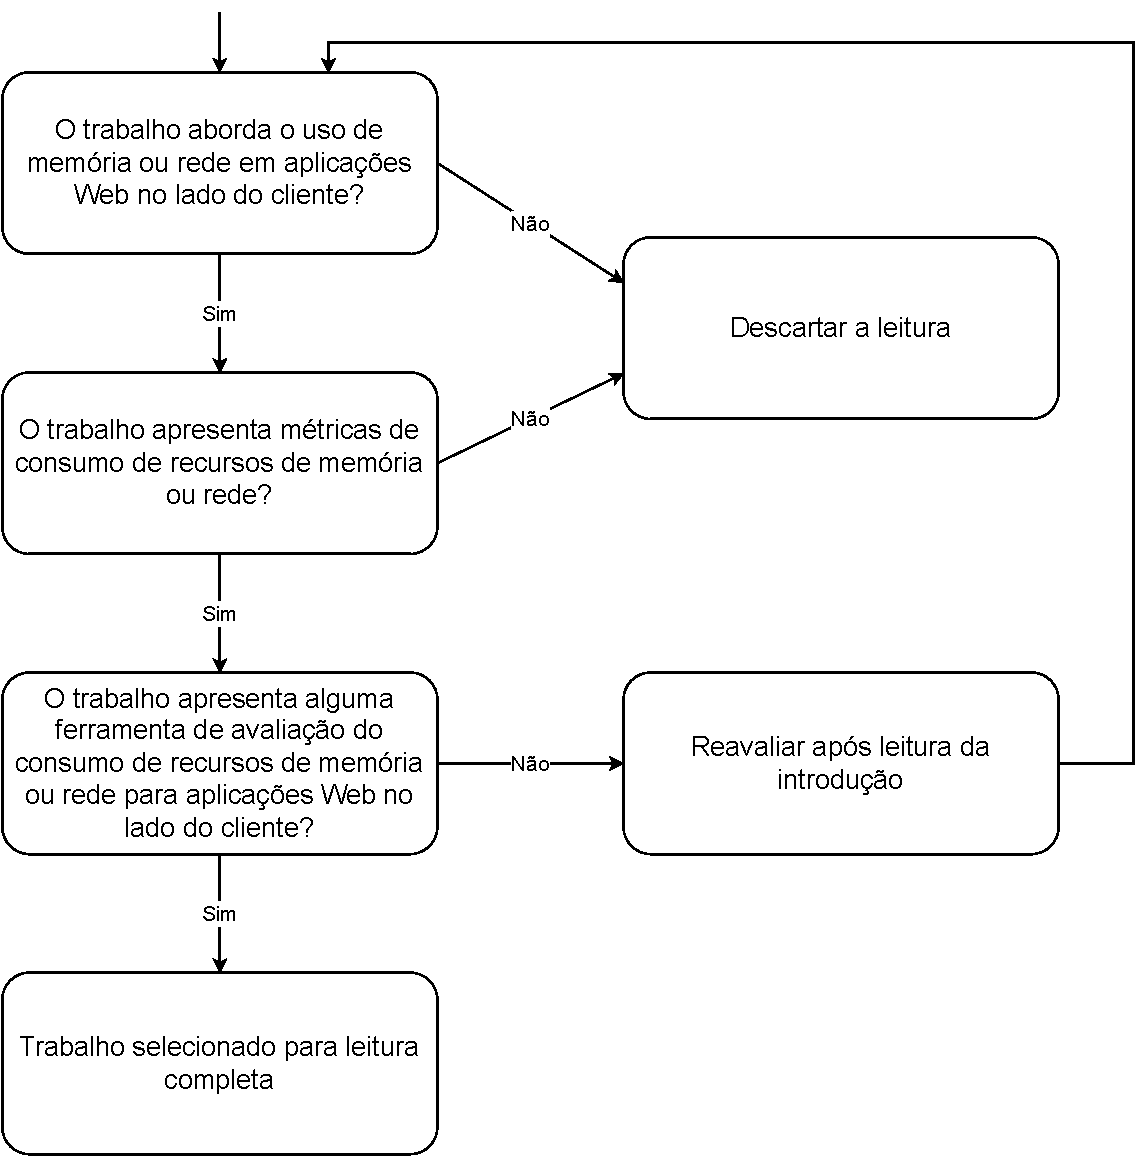
\includegraphics[width=0.6\textwidth]{figures/fluxo-decisao-leitura.pdf}
	\caption{Critérios utilizados para seleção de trabalhos para leitura.}
	\label{fig:fluxo-leitura}
\end{figure}

\begin{table}[!ht]
	\centering
	\caption{Total de trabalhos encontrados}
	\begin{tabular}{l  c L{1.5cm} R{1.5cm}}
		\toprule
		\textbf{Ferramenta} & \textbf{Trabalhos Encontrados} \\
		\midrule
		Elicit  &  280  \\
		Connected Papers  &  120  \\
		\midrule
		Total  &  400  \\
		\bottomrule
	\end{tabular}
	\label{tab:trabalhos-encontrados}
\end{table}

\chapter{Trabalhos Relacionados}
\label{sec:trabalhos_relacionados}
	\label{sec:trab_relacionados}

	% \item \textbf{Paper 1}: Summary of the first paper goes here. This paragraph provides a concise overview of the paper's objectives, methodology, and key findings.
	\section{Ferramentas Para Medição no Lado do Cliente}
	Utilizando os métodos descritos na seção anterior do trabalho, conseguimos levantar um panorama geral dos frameworks e soluções existentes e propostos à academia, assim como classificá-los utilizando alguns parâmetros, afim de entender se a nossa proposta se demonstra complementar ao estado da arte. 
	Os critérios da classificação são: 


	\begin{table}[!ht]
		\centering
		\caption{Critérios de classificação das ferramentas}
		\begin{tabular}{l c L{1.5cm} R{1.5cm}}
			\toprule
			\textbf{Critério} & \textbf{Descrição}\\
			\midrule 
			Arquitetura Simples & Se a arquitetura da ferramenta é de fácil entendimento.\\
			Flexibilidade&Se a ferramenta se adapta em diversos contextos de medição.\\
			Curva de Aprendizado&Se a ferramenta possui uma curva de aprendizado rápida.\\
			Multiplataforma&Se a ferramenta suporta o uso em diversas plataformas.\\
			Persistência&Se a ferramenta persiste dados para análise futura.\\
			\bottomrule
		\end{tabular}
		\label{tab:string-busca-connected-papers}
	\end{table}


	\par Dessa forma, a classificação dos trabalhos selecionados se encontra na tabela abaixo:

		\begin{table}[ht]
			\scriptsize
			\caption{Classificação das ferramentas encontradas} % title of Table
			\centering % used for centering table
			\begin{tabular}{l c c c c c} % centered columns (4 columns)
			\toprule
			\textbf{Plataforma} & \textbf{Arquitetura Simples} & \textbf{Flexibilidade} & \textbf{Curva de Aprendizado} & \textbf{Multiplataforma} & \textbf{Persistência} \\[0.5ex]

			%heading
			\midrule % inserts single horizontal line
			MemInsight & sim & não & sim & sim & não \\
			WePR & não & não & não & sim & sim \\
			Gember & sim & não & sim & não & sim \\
			Mobilyzer & sim & não & não & não & sim \\
			\hline %inserts single line
			\end{tabular}
			\label{table:cls} % is used to refer this table in the text
		\end{table}
	

		\subsection{MemInsight}
		\par No contexto de medição de memória, temos a MemInsight \citep{Jensen2015MemInsight}. Essa ferramenta roda de forma independente sobre uma engine Javascript, não sendo necessário um browser para executar, e faz a análise do consumo de memória por meio de um conjunto de medições que visam remontar o ciclo de vida dos objetos em memória, e que permitem a análise de desperdício de recursos durante a execução do programa. 
		\par Analisando a ferramenta, foi observado que ela só trabalha com medição de métricas de memória, não permitindo generalizar consultas de outros tipos, por isso classificamos como não flexível com relação às métricas. Além disso, por ser uma ferramenta com foco em depurar aplicações, não realiza nativamente a persistência e organização desses dados.
		

		\subsection{WePR}
		\par \citep{Asrese2019MeasuringWL} também propôs uma ferramenta para medição no lado do cliente, porém agora com o enfoque em medir métricas de \acr{QoS}, nomeada WePR. No trabalho, ele apresenta um panorama da evolução da web, especialmente de como a latência se desenvolveu nos sites, e sustenta a necessidade desse tipo de medição como forma de melhorar a experiência do usuário, que indicam ser um fator determinante no abandono ou sucesso de um website. A ferramenta foi testada utilizando grandes sites como Google, Youtube e Facebook. 
		\par A arquitetura da ferramenta é distribuída, e consiste basicamente de um coletor, um servidor que fornece os elementos das páginas para medição, múltiplos servidores de renderização gerenciados por um balanceador de carga (do inglês, \emph{load balancer}), e um servidor que cuida da persistência dos dados. Dessa forma, o coletor inicialmente pede ao servidor as URLs dos elementos a serem medidos, e após obter essa resposta, faz o download desses elementos e captura métricas. Posteriormente, envia esses dados medidos e os elementos baixados para o balanceador de carga, e por fim algum dos servidores de renderização envia os dados para persistência.
		\par O enfoque da ferramenta é a análise de desempenho de sites, dessa forma sua arquitetura e usabilidade não foram construídas de forma simples de estender, tornando difícil a utilização da ferramenta em outros contextos. Além disso, não temos a possibilidade de incluir métricas customizadas, o que torna sua análise pouco flexível.
		
		\subsection{Gember}
		\par \citep{Gember2012Obtaining} também traz um estudo sobre medição no lado do cliente, porém dessa vez em clientes móveis, utilizando dados de um provedor de internet e também de experimentos controlados. Esse tipo de medição é muito útil para provedores de internet e desenvolvedores, que precisam entender como suas aplicações se saem interagindo com redes móveis de internet.
		\par Foi desenvolvido no trabalho um protótipo para Android de um medidor de performance para analisar somente quando o dispositivo está ativo, e que é integrado ao app como uma biblioteca. A arquitetura consiste basicamente de um controlador central (servidor), e múltiplos clientes (aparelhos) com o código rodando em seus celulares. Dessa forma, o pesquisador faz uma requisição para esse controlador, e ele coordena a coleta do que foi solicitado nos aparelhos, salvando os resultados no servidor.
		\par O serviço inicialmente coleta latência, taxa de transferência (do inglês, {throughput}) e o tempo de carregamento de páginas Web, é extensível para outras métricas de rede, porém limitado a elas. Outra limitação aqui é a utilização no cliente, que se encontra somente no sistema operacional Android, tornando pouco flexível a utilização dessa ferramenta nos contextos de pesquisas multiplataforma.

		\subsection{Mobilyzer}
		\par Ainda no contexto de medição de rede, se encontra o Mobilyzer \citep{Nikravesh2015Mobilyzer}, uma plataforma aberta para medição de rede em dispositivos móveis. Essa plataforma foi criada com o objetivo de prover uma solução escalável, eficiente e controlável, que fosse possível de ser incorporada tanto a apps em desenvolvimento, quanto em apps que já estão desenvolvidos, para suportar pesquisas e testes em medição de rede. 
		\par Ela funciona utilizando alguns componentes básicos, sendo eles: 
		\begin{enumerate}
			\item Uma biblioteca Android, que é integrada aos aplicativos para coletar as informações e enviar ao servidor. Ela é incorporada direto no código fonte.
			\item Um componente chamado gerenciador de memória, no qual o pesquisador pode inserir medições de forma customizada e mais eficiente. Ele também realiza o agendamento das medições, e também coordena e monitora os dispositivos para que não tenha sobrecarga em nenhum aparelho ou rede medida. 
			\item Um servidor na nuvem, que fica responsável por coletar, analisar aplicando regras e publicar os dados coletados dos dispositivos. Essa arquitetura centralizada simplifica o compartilhamento de dados entre essas etapas, podendo integrar outras ferramentas de análise de dados com a base das coletas.

		\end{enumerate}
		\par Uma dificuldade no uso do Mobilyzer em pesquisas é que essa plataforma também se restringe a plataforma Android. Diminuindo bastante as possibilidades de medição em pesquisas multiplataforma. Além disso, não possui muita flexibilidade com relação às métricas, sendo em sua maior parte métricas de rede.

		\subsection{Nossa Ferramenta}
		\par Após o descrito, podemos posicionar a nossa ferramenta com relação aos critérios que estabelecemos no começo desta seção. Temos um modelo de arquitetura simples que será explicado nas seções futuras deste trabalho, a possibilidade de expandir e construir métricas diversas, uma curva de aprendizado suave, a compatibilidade com múltiplas plataformas pois a coleta das métricas ocorre no navegador, e também a persistência desses dados para futura análise.
		\par Assim, a tabela teria a seguinte configuração após a adição da nossa ferramenta:

		\begin{table}[ht]
			\scriptsize
			\caption{Classificação das ferramentas encontradas com a nossa ferramenta} % title of Table
			\centering % used for centering table
			\begin{tabular}{c c c c c c} % centered columns (4 columns)
			\toprule %inserts double horizontal lines
			\textbf{Plataforma} & \textbf{Arquitetura Simples} & \textbf{Flexibilidade} & \textbf{Curva de Aprendizado} & \textbf{Multiplataforma} & \textbf{Persistência} \\[0.5ex]

			%heading
			\midrule % inserts single horizontal line
			MemInsight & sim & não & sim & sim & não \\
			WePR & não & não & não & sim & sim \\
			Gember & sim & não & sim & não & sim \\
			Mobilyzer & sim & não & não & não & sim \\
			Nossa Ferramenta & sim & sim & sim & sim & sim \\
			\bottomrule %inserts single line
			\end{tabular}
			\label{table:nonlin} % is used to refer this table in the text
		\end{table}

\chapter{Proposta}
\label{cap:proposta}

O objetivo do framework é oferecer uma forma fácil e eficaz de realizar análises de desempenho e consumo de recursos computacionais em provas de conceito para aplicações Web no lado do cliente.
De modo que, o usuário do framework seja capaz de realizar suas análises com a colaboração de voluntários, sendo o framework responsável pela coleta e agregação das métricas em uma base de dados.
A fim alcançar estes objetivos, o trabalho se divide em três fases: pesquisa, implementação e experimentação.

Durante a fase de pesquisa, há o levantamento da bibliografia, inicio do desenvolvimento da fundamentação teórica e busca por trabalhos semelhantes.
A fase de implementação, por sua vez, se divide em três etapas principais: (i) planejamento e documentação, (ii) ensaio dos conceitos e (iii) implementação do artefato.
Posteriormente, a solução implementada é aplicada a um experimento de seu uso, para avaliação de usabilidade e documentação de uso.

\begin{figure}[!ht]
	\centering
	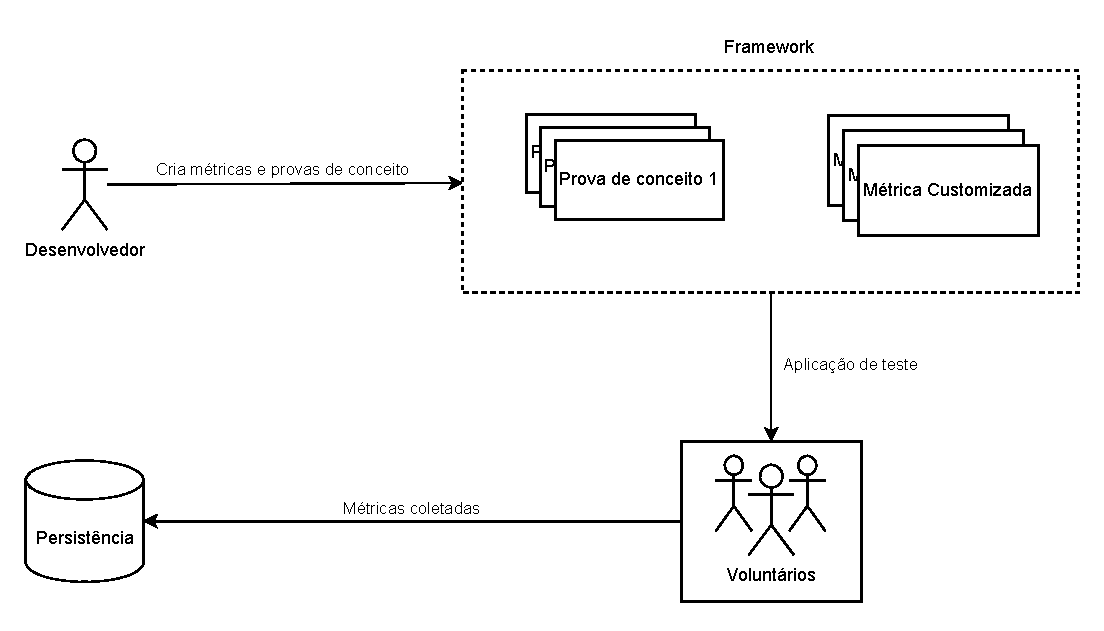
\includegraphics[width=0.6\textwidth]{figures/diagrama-informal.pdf}
	\caption{Principal fluxo de uso, onde um desenvolver avalia um conjunto de provas de conceitos com o auxílio de voluntários externos ao desenvolvimento.}
	\label{fig:diagrama-informal}
\end{figure}

\section{Planejamento e Documentação}
\label{sec:planejamento-doc}

Esta etapa tem como objetivo definir como os objetivos do framework são alcançados.
Para tanto, nela são gerados dois artefatos: o diagrama conceitual (figura \ref{fig:diag-conceitual}) e o diagrama de classes (figura  \ref{fig:diag-classes}).
Primeiro, o diagrama conceitual é desenvolvido com o objetivo de elaborar as principais ideias as quais definem o funcionamento do framework.
Enquanto, o diagrama de classes tem como objetivo evidenciar os aspectos práticos de seu desenvolvimento e planejar os módulos de sua arquitetura.

\subsection{Diagrama Conceitual}

\begin{figure}[!ht]
	\centering
	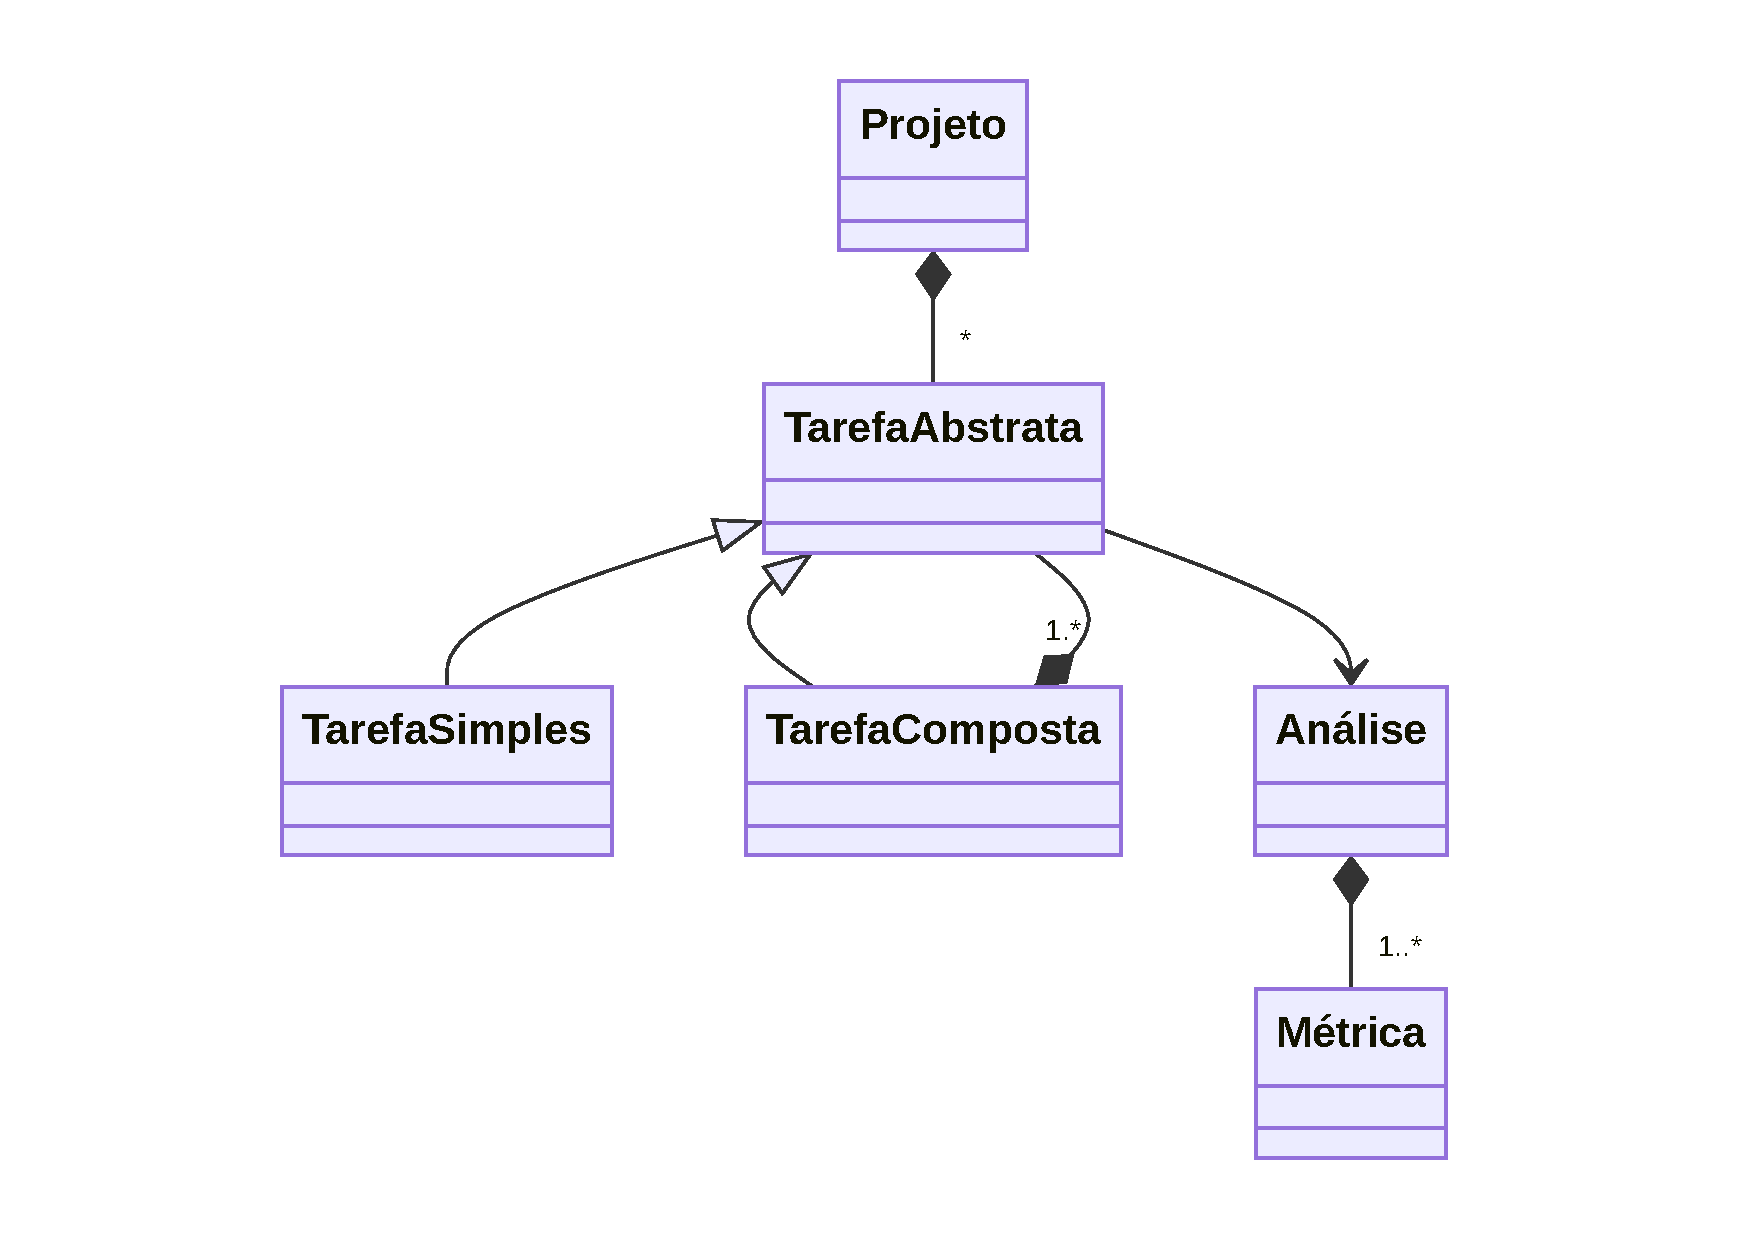
\includegraphics[width=0.6\textwidth]{figures/diagrama-conceitual.pdf}
	\caption{Diagrama conceitual do framework.}
	\label{fig:diag-conceitual}
\end{figure}

O diagrama conceitual define como o framework é estruturado, nele há a fundação do framework em ser um aplicativo modelo, o qual o usuário gera a versão final ao adicionar tarefas concretas.
Estas tarefas representam as provas de conceito, de modo que, um artefato gerado pelo framework seja capaz de conter mais de uma prova de conceito para avaliação.
Além disso, outra definição importante do diagrama conceitual é a utilização do padrão de projeto Composite \citep{Gamma1995Design} para permitir a avaliação de etapas das provas de conceito.
Abaixo, está uma descrição de cada elemento do diagrama conceitual.

\begin{description}
	\label{descrip:diagrama-conceitual}

	\item[Projeto:] Representa a aplicação a qual pertence as provas de conceito. Além disso, também é o principal objeto do framework, por conter a referência para a raíz das árvores de \textit{Tarefas} e coordenar a execução das avaliações.
	
	\item[Tarefa Abstrata:] Representa um procedimento para ser executado pelo framework. Ou seja, representa uma etapa ou prova de conceito integral que está sob avaliação.

	\item[Tarefa Simples:] Representa os containers que recebem o código das provas de conceito.

	\item[Tarefa Composta:] Representa um grupo de provas de conceito ou uma prova de conceito decomposta em etapas.

	\item[Análise:] Representa um conjunto de métricas de avaliação de um procedimento abstrato. Ou seja, todas as tarefas as quais são implementações diferentes de um mesmo procedimento podem compartilhar a mesma análise.

	\item[Métrica:] Representa uma medida quantitativa de algum recurso despendido durante a execução de uma \textit{Tarefa}.

\end{description}


\subsection{Diagrama de Classes}

\begin{figure}[!ht]
	\centering
	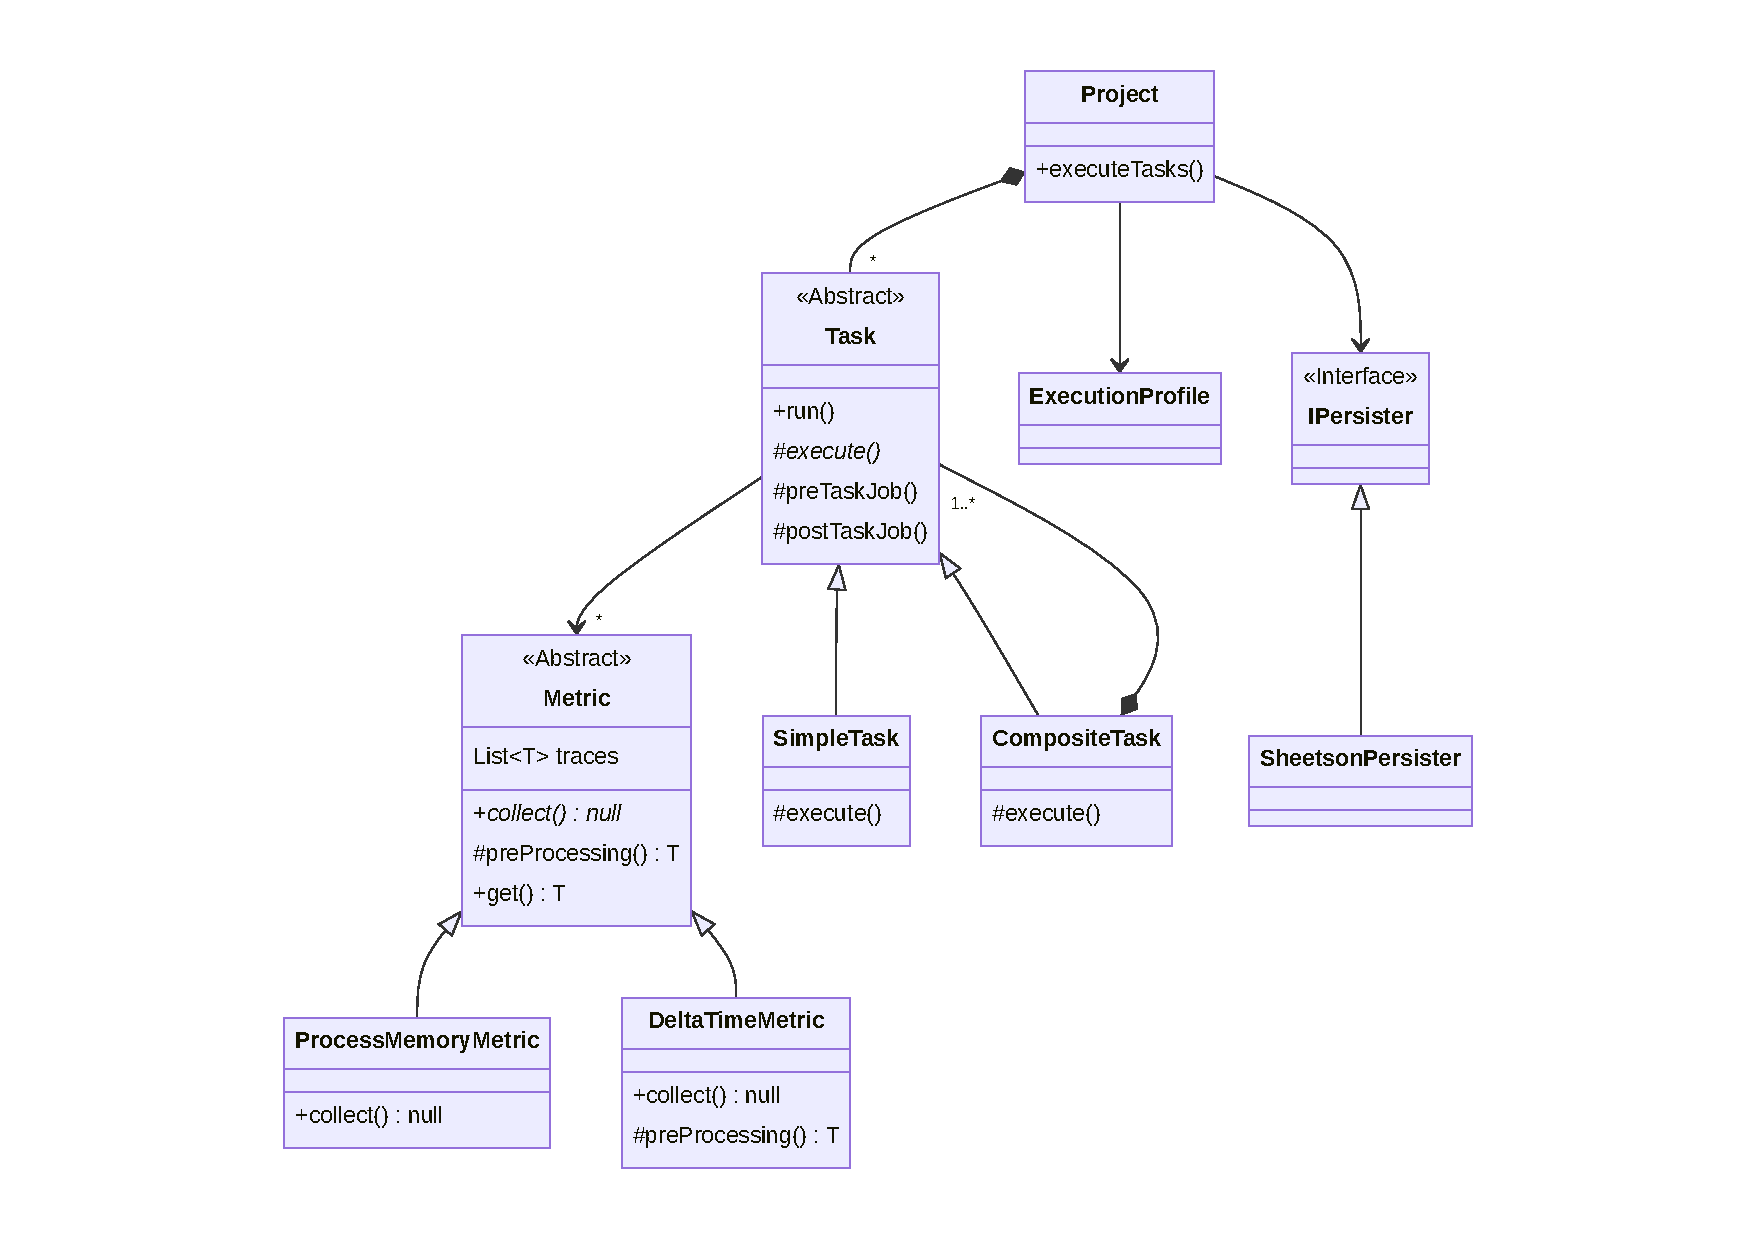
\includegraphics[width=0.9\textwidth]{figures/diagrama-classes.pdf}
	\caption{Diagrama classes do framework.}
	\label{fig:diag-classes}
\end{figure}

O diagrama de classes define a arquitetura e estrutura dos módulos do framework.
Nele há a definição dos principais aspectos práticos para a implementação, por exemplo, são definidas as árvores de herança e principais métodos que precisam ser implementados por usuários.
Além disso, ele também define a camada de persistência para resolver o problema da coleta de métricas de execuções realizadas por voluntários de forma remota.
Abaixo, está uma descrição de cada elemento do diagrama.

\begin{description}
	\item[Project:] Responsável por coordenar a execução das análises e encaminhar suas métricas para a camada de persistência.
	\item[ExecutionProfile:] Responsável pela coleta de dados sobre o ambiente de execução.
	\item[Task:] Responsável por definir a rotina de execução das tarefas e seus métodos públicos.
	\item[SimpleTask:] Classe base para implementação de uma tarefa.
	\item[CompositeTask:] Classe base para implementação de tarefas compostas.
	\item[Metric:] Responsável por definir a rotina para coleta de uma métrica e seus métodos públicos.
	\item[ProcessMemoryMetric:] Implementação de uma métrica para medir o consumo de memória.
	\item[DeltaTimeMetric:] Implementação de uma métrica para medir tempo gasto em uma tarefa.
	\item[IPersister:] Responsável por definir a interface pública da camada de persistência.
	\item[SheetsonPersister:] Implementação da camada de persistência a qual utiliza o Google Sheets\footnote{https://www.google.com/sheets/about}.
\end{description}

Como foi anunciado anteriormente, realizar a coleta de métricas em execuções realizadas por voluntários, os quais podem atuar de modo remoto é um problema destacado pelo diagrama de classes.
Pois, em uma abordagem convencional construiríamos uma \acr{API} com arquitetura REST (do inglês, \emph{representational state transfer}) para receber as métricas e disponibilizá-las para consulta.
Ademais, também haveria a necessidade de implementar uma camada de autorização na \acr{API} para prover segurança aos dados dos usuários.
Entretanto, esta abordagem possui sérias desvantagens, sendo as duas principais: um aumento considerável no escopo de implementação e custos com infraestrutura para a \acr{API}.

Portanto, optamos por uma outra abordagem para persistência das métricas.
Nela o framework utiliza o Google Sheets como forma de armazenamento e visualização das métricas das execuções.
Para tanto, ao invés de desenvolver uma \acr{API}, usamos a própria \acr{API} do Google Sheets, ao custo de requerer que o usuário do framework possua uma conta Google.
Porém, a \acr{API} do Google Sheets não atende diretamente as necessidades do framework, devido ao fato de exigir um cadastro da aplicação, mas com uso da ferramenta Sheetson\footnote{https://sheetson.com} não há essa limitação.


\chapter{Prova de conceito}
\label{cap:prova_de_conceito}
A fim de testar a modelagem proposta, desenvolvemos uma prova de conceito com objetos mock, os quais simulam recursos computacionais.
De modo que fosse possível avaliar a eficácia da modelagem sem depender de recursos físicos reais, visando manter o foco na estrutura do framework.
A prova de conceito foi implementada usando a linguagem de programação Typescript, sua escolha almeja expressar com clareza todas as classes e relações definidas durante a modelagem, e seu código-fonte pode ser encontrado no apêndice \ref{apx:mock_source}.


\section{Simulação de Recursos Computacionais}
Como mencionado anteriormente, a prova de conceito possui classes para simular recursos computacionais.
As quais possuem a finalidade de isolar a prova de conceito de complexidades inerentes a realização de medições reais.
Logo, o desenvolvimento da prova de conceito pode ser concentrado em explorar o ponto central da modelagem, a árvore de \emph{Tarefas}.
O bloco de código \ref{lst:mock_memoria} contém a classe criada para simular o consumo de memória.

\begin{lstlisting}[label={lst:mock_memoria}, caption={Implementação da classe responsável por simular recursos de memória para a prova de conceito do framework.}, language=TypeScript]
class Resource {
    private static _total: number = 500;

    static alloc(size: number): any {
        this._total -= size;
        return {size};
    }

    static free(block: any): void {
        this._total += block.size;
    }

    static get total(): number {
        return this._total;
    }
}
\end{lstlisting}


\section{Árvore de Tarefas}

A árvore de tarefas é definida basicamente por três classes:
a classe abstrata \emph{Task}, responsável por definir o que uma tarefa faz, ou seja, a sua interface pública.
A classe \emph{CompositeTask}, a qual possui a função de agregar outras tarefas.
E, a classe \emph{SimpleTask}, responsável por encapsular e executar o código do usuário do framework.
Entretanto, tanto \emph{CompositeTask} quanto \emph{SimpleTask} servem apenas para fins de herança e polimorfismo.
Portanto, com o framework em sua completude, as derradeiras classes, as quais compõem a árvore de tarefas, serão subclasses.

\begin{lstlisting}[label={lst:abstract_task}, caption={Classe abstrata responsável por definir o que todos os membros da árvore de tarefas precisam implementar.}, language=TypeScript]
abstract class Task {
    public name: string;
    public metrics: Set<Metric<any>>;

    constructor(name: string, metrics: Metric<any>[])
    {
        this.metrics = new Set(metrics);
        this.name = name;
    }

    async run(): Promise<any> {
        this.preTaskJob();
        let data = await this.execute();
        let metrics = {};
        this.metrics.forEach(element => {
        metrics[element.name] = element.metric;
        });
        this.postTaskJob();
        return {metrics, data};
    }

    preTaskJob(): void {};
    abstract execute(): Promise<any>;
    postTaskJob(): void {};
}
\end{lstlisting}

\begin{lstlisting}[label={lst:composite_task}, caption={Tarefa composta, define o comportamento de todos os nós não folha da árvore de tarefas.}, language=TypeScript]
export class CompositeTask extends Task {
    private tasks: Task[];

    constructor() {
        super("Composite Task", []);
        this.tasks = [];
    }

    addTask(task: Task): void {
        this.tasks.push(task);
        task.metrics.forEach(element => {
            this.metrics.add(element);
        });
    }

    async execute(): Promise<any> {
        console.log("Executing composite task...");
        let tasks = {};
        for (const task of this.tasks) {
            tasks[task.name] = await task.run();
        }
        return tasks;
    }
}
\end{lstlisting}


\section{Como executar}
Para utilizar essa prova de conceito, basta criar um arquivo, criar suas tarefas, organizá-las usando as tarefas compostas e criar um Projeto passando a tarefa principal, que vai ser a raiz da árvore, e por fim executar a aplicação. Após isso será criado um arquivo JSON com o resultado da análise das tarefas.
Segue o exemplo de uso:
\begin{lstlisting}[language=TypeScript]
class Index {
	public static async main() {
		console.log("Hello world!");
		const task = new CompositeTask();
		const task2 = new CompositeTask();
		task.addTask(new MockTask("Task 1"));
		task.addTask(new MockTask("Task 2"));
		task2.addTask(new MockTask("Task 3"));
		task.addTask(task2);
		const project = new Project(
			new BasicPersister(),
			task);
		project.executeTask();
	}
}
\end{lstlisting}
Nesse caso foi criado uma tarefa composta chamada task, que tem duas tarefas simples e uma outra tarefa composta chamada task2, que tem uma tarefa simples. A task2 foi adicionada a task, e por fim a task foi adicionada ao projeto. Após isso foi executado o projeto, que vai executar todas as tarefas e gerar o arquivo JSON com o resultado da análise.

\section{Exemplo de uso}
Um exemplo ilustrativo de uso do framework consiste em comparar o desempenho de consultas em dicionários e listas, a fim de determinar qual estrutura de dados oferece melhor desempenho em termos de velocidade e uso de memória. Vamos explorar esse exemplo para ilustrar a funcionalidade da prova de conceito.

Primeiramente, é necessário verificar se todas as métricas necessárias para a avaliação estão implementadas. Caso alguma métrica esteja ausente, é possível criá-la estendendo a classe de métrica abstrata e implementar a lógica específica para gerar essa métrica. Nesse exemplo, vamos analisar o uso de memória e o tempo de execução. Como essas métricas já estão implementadas, não é necessário criar novas métricas para essa comparação.

Após garantir a disponibilidade das métricas, podemos implementar as tarefas que serão avaliadas: uma que trabalha com listas e outra que utiliza dicionários. Nesse caso, como estamos realizando uma prova de conceito, faremos uso de um objeto mock para a memória, que simula a alocação e desalocação de memória, e da função que espera um tempo aleatório, que simula o tempo de execução de uma tarefa.

Uma vez implementadas as tarefas, podemos criar um arquivo chamado ``index.ts''. Nele, criaremos uma CompositeTask que incluirá as duas tarefas previamente implementadas: a tarefa com dicionários e a tarefa com listas. Em seguida, criaremos um novo projeto, passando a CompositeTask como parâmetro para a sua execução. Esse projeto será responsável por salvar os resultados em um arquivo específico.

Por fim, poderemos analisar os resultados salvos no arquivo para determinar qual implementação se mostra mais adequada para a nossa aplicação, considerando o desempenho apresentado pelas estruturas de dados em termos de velocidade e uso de memória. Ao realizar esse exemplo, aproveitamos as capacidades da prova de conceito para comparar o desempenho de diferentes estruturas de dados, auxiliando na tomada de decisões informadas e na seleção da melhor abordagem para otimizar a nossa aplicação.

\chapter{Estado Atual do Trabalho}
\label{cap:estado_atual}

Com a definição do framework e seu escopo em mãos, realizamos a pesquisa a qual origina o capítulo \ref{cap:met_pesquisa}.
Tendo como objetivo, confirmar se há espaço dentro do ecossistema das ferramentas de análise de desempenho e recursos computacionais para o que estamos propondo.
Como dentre as ferramentas encontradas não havia uma voltada para que um desenvolvedor seja capaz de avaliar provas de conceito de modo customizável em diversos tipos de configurações do lado do cliente, concluímos que há espaço para a proposta do nosso framework.

Após isso, o próximo passo foi a definição dos conceitos do framework.
Para tanto, elaboramos o diagrama conceitual o qual tem o papel de definir como os objetivos do framework devem ser alcançados e planejar as principais características da arquitetura do projeto.
Por exemplo, nessa etapa foi onde definimos que o padrão de projeto Composite seria utilizado, com o objetivo de permitir que uma prova de conceito seja dividida em etapas as quais possuem suas próprias métricas.
Deste modo, fica a critério do usuário se sua abordagem trata as provas de conceito como um bloco único ou como um conjunto de etapas, o que pode permitir diagnósticos de desempenho mais precisos.

O terceiro passo foi voltado para a arquitetura do projeto.
Onde elaboramos o diagrama de classes e avaliamos os principais aspectos práticos de seu desenvolvimento.
Dentre eles, o ponto de maior destaque foi como realizar a captura das métricas de execuções realizadas por voluntários.
Pois, uma abordagem tradicional ao problema envolveria o desenvolvimento de uma \acr{API} para nos permitir receber e disponibilizar a consulta dos dados.
Entretanto, disponibilizar os dados dos usuários do framework na Internet tornaria necessário também criar uma camada de autorização, expandindo ainda mais o escopo de desenvolvimento.
A solução encontrada para o problema foi a utilização do programa de planilhas online Google Sheets, onde ao invés da execução do framework enviar as métricas para uma \acr{API} nossa, ela envia para uma planilha do próprio usuário.
Deste modo, não há a necessidade do desenvolvimento de \acr{API}, pois, utilizamos uma do Google Sheets e o controle de acesso aos dados também fica sob responsabilidade deles.

A última etapa atual está sendo o desenvolvimento de uma prova de conceito do próprio framework.
Para tanto, optamos por desenvolver utilizando a linguagem de programação TypeScript, a fim de exercitar as classes e relações planejadas durante a criação dos diagramas.
Nela estamos utilizando objetos mock, a fim de simular comportamentos do ambiente como consumo de memória e tempo gasto na execução de tarefas.
Além de simular como um usuário do framework aplicaria a estrutura de árvore de tarefas em suas provas de conceito.
Durante essa etapa também encontramos algumas limitações do conceitos como a inaplicabilidade do conceito de análise como uma avaliação independente de tarefas, pois, seria necessário restringir a liberdade na obtenção de métricas.

O desenvolvimento do framework e produção textual estão sendo realizados em paralelo.
A fundamentação teórica e critérios para comparação do framework com outras ferramentas tem conclusão prevista para outubro de 2023.
A descrição do framework, capítulo \ref{cap:proposta}, será realizada de forma mais precisa e detalhada até janeiro de 2024, junto com um exemplo de sua utilização.
A defesa da dissertação está prevista para janeiro de 2024. O cronograma indicado na tabela \ref{tab:cronograma} prevê as etapas abordadas neste trabalho.
A tabela indica os meses de previsão de conclusão de cada uma das etapas.

\begin{table}[!ht]
	\centering
	\caption{Cronograma de desenvolvimento da dissertação}
	\begin{tabular}{l  c  c  c  c  c  c L{1.5cm} R{1.5cm}}
		\toprule
		\textbf{Atividade} & \textbf{fev-mar} & \textbf{abr-mai} & \textbf{jun-jul} & \textbf{ago-set} & \textbf{out-nov} & \textbf{dez-jan} \\
		\midrule
		Planejamento e Escopo  &  X  &    &    &    &    &    \\
		Fundamentação Teórica  &  X  &     &    &  X  &    &    \\
		Arquitetura  &    &  X  &  X  &    &    &    \\
		Prova de Conceito  &    &    &  X  &    &    &    \\
		Desenvolvimento  &    &    &  X  &  X  &  X  &    \\
		Exemplo de Uso  &    &    &    &    &  X  &  X  \\
		Defesa  &    &    &    &    &    &  X  \\
		\bottomrule
	\end{tabular}
	\label{tab:cronograma}
\end{table}

\label{bibpage}
\renewcommand\bibname{Referências}
\addcontentsline{toc}{section}{Referências}
\bibliography{references}
%\bibliographystyle{plainnat}
\bibliographystyle{apalike}
\label{bibfinalpage}

\label{lastpage}


\appendix
\chapter{Código-fonte da Prova de Conceito}
\label{apx:mock_source}

\section{Projeto}
\lstinputlisting[language=TypeScript]{./mock/Project.ts}

\section{Index}
\lstinputlisting[language=TypeScript]{./mock/Index.ts}

\section{Tarefa Abstrata}
\lstinputlisting[language=TypeScript]{./mock/Tasks/Task.ts}

\section{Tarefa Composta}
\lstinputlisting[language=TypeScript]{./mock/Tasks/CompositeTask.ts}

\section{Tarefa Simples}
\lstinputlisting[language=TypeScript]{./mock/Tasks/SimpleTask.ts}

\section{Exemplo de implementação de tarefa}
\lstinputlisting[language=TypeScript]{./mock/Tasks/MockTask.ts}

\section{Interface de persistencia}
\lstinputlisting[language=TypeScript]{./mock/Persister/IPersister.ts}

\section{Exemplo de persistencia}
\lstinputlisting[language=TypeScript]{./mock/Persister/BasicPersister.ts}

\section{Mock de tempo}
\lstinputlisting[language=TypeScript]{./mock/Helpers/MockTime.ts}

\section{Mock de Memoria}
\lstinputlisting[language=TypeScript]{./mock/Helpers/MockResource.ts}

\section{Metrica abstrata}
\lstinputlisting[language=TypeScript]{./mock/Metrics/Metric.ts}

\section{Metrica de tempo}
\lstinputlisting[language=TypeScript]{./mock/Metrics/GetDeltaTime.ts}

\section{Metrica de memoria}
\lstinputlisting[language=TypeScript]{./mock/Metrics/GetResourceUsage.ts}

\end{document}